\chapter{Seeking more robust early warning signals for climate tipping points: the Ratio of Spectra method (ROSA)}
\graphicspath{{ROSA/figs}}


 Potential tipping points in the Earth System present challenges for society and 
ecosystems, especially as the global warming thresholds at which these may be triggered remain uncertain. 
Fortunately, a theory of `critical slowing down' has been developed which could warn of approaching tipping points. 
Applications of this theory often implicitly assume stationary white-noise forcing,  itself requiring a clean separation between forced trends and variability, which is especially difficult under contemporary climate change. 
This paper proposes a modified method to derive early warning signal in a 
system, such as the climate, which is forced by time correlated processes. 
The method looks at the \emph{Ratio of Spectra (ROSA)} of a system state variable relative to a forcing variable.   
We demonstrate the ROSA method on an idealised forced dynamical system, before applying it 
to a particular challenging example from the Earth System: dieback of the Amazon rainforest. We show that ROSA identifies more examples of abrupt transitions in the Amazon than conventional early warning signals in state-of-the-art CMIP6 Earth System Models.


\section{Introduction}\label{sec:introduction}
The paleoclimate record contains numerous examples\cite{Brovkin2021} of 
major components of the Earth system experiencing rapid 
change. Such changes can be caused by 
relatively small changes in external forcing, such as changes in incoming
solar radiation or in greenhouse gas concentrations.

Over the last two hundred years humans have increasingly forced the climate system, 
primarily through the burning of fossil fuels,
which has caused global warming and other related changes to the climate
system. As a result there is now major scientific interest and public 
concern\cite{Lenton2019a,Steffen2018,Ritchie2021}
that future 
temperature increases may also cause key
Earth System components (so called `Tipping Elements')  to cross 
critical thresholds known as `Tipping Points', undergoing rapid 
irreversible transitions\cite{Lenton2008}. 

Tipping points are typically triggered by a small change in a system parameter, such as one describing the forcing or relating to aspects of the internal structure. Crossing some critical threshold associated with this parameter causes the system to be pushed into a qualitatively 
different state. Mathematically this can be described as a system passing through a bifurcation. 
Although different types of tipping exist\cite{Ashwin2012}, in the analysis here 
we will be concerned with so-called `Bifurcation-' or `B-tipping'.


Pioneering work by Stommel suggested that the Atlantic Meridional Overturning 
Circulation (AMOC)\cite{STOMMEL1961} is such a tipping element, although
his work predates widespread use of the term. Since then,
numerous examples of potential tipping elements have been identified.
For example, the Amazon Rainforest can undergo dieback\cite{Cox2000}, the 
Greenland ice-sheet can melt\cite{Feldmann2015} and
permafrost can thaw rapidly\cite{Steffen2018}.

Sophisticated climate model simulations\cite{Rahmstorf1995} provide evidence that tipping points can occur in the Earth System.
For example, multiple
instances of abrupt shifts were identified in the Coupled Model Intercomparison Project - Phase 5 (CMIP5)\cite{Taylor2012}
collection of Earth System Models (ESMs)\cite{Drijfhout2015} and hysteresis has been found in 
simulations of the Antarctic Ice Sheet\cite{Garbe2020}. 

It is unsurprising that major transitions in important components
of the Earth System would have significant impacts. As tipping points
are not routinely included in Integrated Assessment Models (IAMs) many of 
their impacts on society are not yet quantified, yet recent 
work\cite{Dietz2021}
suggests including tipping points in IAMs
substantially increases the Social Cost 
of Carbon. Impact studies of individual 
Tipping Points reveal significant challenges for many people. For instance, a 
collapse of the AMOC is projected to cause
widespread cessation of arable farming in Great Britain\cite{Ritchie2020a}.
High latitude communities face increased fire risks caused 
by the self-heating of soils\cite{Clarke2021} and infrastructure damage 
caused by a rapid increase in permafrost degradation\cite{Teufel2019}. 


Given the potential for major impacts, it would be useful to know the exact thresholds of
these tipping points, however precision remains elusive\cite{Steffen2018}.
There is almost no inter-ESM
agreement on which tipping points are the most likely to happen, or on the
levels of global warming that will trigger their
occurrence \cite{Drijfhout2015}.
However due to the mathematical theory of Normal 
Forms\cite{Strogatz2015,guckenheimer2013}, all systems approaching a
B-tipping point share some common features.

For our purposes, the most important of these generic characteristics
is \emph{critical slowing down}. Systems generally revert to  equilibrium after a small disturbance. 
The time to return to equilibrium is a characteristic timescale which, importantly, increases as the system 
approaches a tipping point, at which moment the timescale becomes 
infinite\cite{Scheffer2012}---referred to as `critical slowing down'. 
For near-equilibrium systems, the variance of a system will increase and its autocorrelation (AC)
will tend to unity as the system approaches a bifurcation\cite{Scheffer2009,Held2004}. These statistical changes lead to the possibility of `Early Warning Signals' (EWS) of approaching Tipping Points.

Care is needed when using EWS, as we 
expect both AC and variance to increase as a tipping point is 
approached\cite{Ditlevsen2010}. Whilst this is only strictly true
in the case of near one dimensional systems (an approximation which is often made, such as by using principle component analysis to reduce the 
dimensionality of the system\cite{Held2004}), considering one quantity alone 
increases the chance of a false positive as that quantity may change for other reasons such as an increase in the noise variability. It should 
be noted that false positives can still occur even when considering 
both quantities.
%could instead be changing because the system's environment is changing.
Additionally, 
%one must be confident the transition is bifurcation induced, 
%rather than noise induced (`N-tipping'). In the N-tipping case, 
if a transition is noise-induced (rather than bifurcation-induced) then
critical
speeding up is possible, where
%, leading to 
a decrease in the variance and AC can
be signs of an approaching transition\cite{Titus2020}.

The technique of observing an increase in the variance and
AC has been applied to the paleoclimate record, where it has been shown to give early
warnings of tipping points\cite{Boers2018a}. It has also been used to 
suggest that for the present day, due to an increase in global temperatures, we are approaching tipping points in 
the Greenland Ice Sheet\cite{Boers2021} and in the AMOC\cite{Boers2021a}.	
However, a key assumption when using the variance and AC as EWS is that the system is subject to a statistically stationary white-noise forcing. Unfortunately, for many
components of the Earth System, the external drivers do not have variability that exhibits white noise characteristics, and
so this assumption is not satisfied. For example, forcing factors in the Earth System are rarely well approximated by stationary white-noise, due to the many quasi-oscillatory modes
of variability in the Earth System\cite{VonderHeydt2021}, which add peaks
to the power spectrum of the forcing. For example, the Amazon
Rainforest, which is of particular interest due to its risk of large-scale vegetation dieback in a potentially hotter and drier
climate, experiences
forcing which is coherent in space and in time, but is also strongly modulated by the
El-Ni\~{n}o Southern Oscillation (ENSO)\cite{Jimenez-Munoz2016}.
White noise forcing is also incompatible with
long memory processes\cite{Hurst1957}, such as the effect of sea ice changes on the AMOC\cite{Kuehn2021}. Recently, it was shown\cite{Kuehn2021}
that traditional EWS  can change their characteristics or disappear entirely when we relax these assumptions on the forcing. This motivates creating EWS that do not assume white noise.


There has been some investigations in using EWS with time correlated noise using generalised least squares\cite{Boers2021a,Boettner2022} and a Bayesian method\cite{hessler2022,Hessler2022b}. Here we examine a 
different method of estimating the critical slowing down that occurs near
a bifurcation that works even in the presence of time-correlated noise.

\section{Failure of Early Warning Signals}
\label{sec:failure}
\begin{figure}
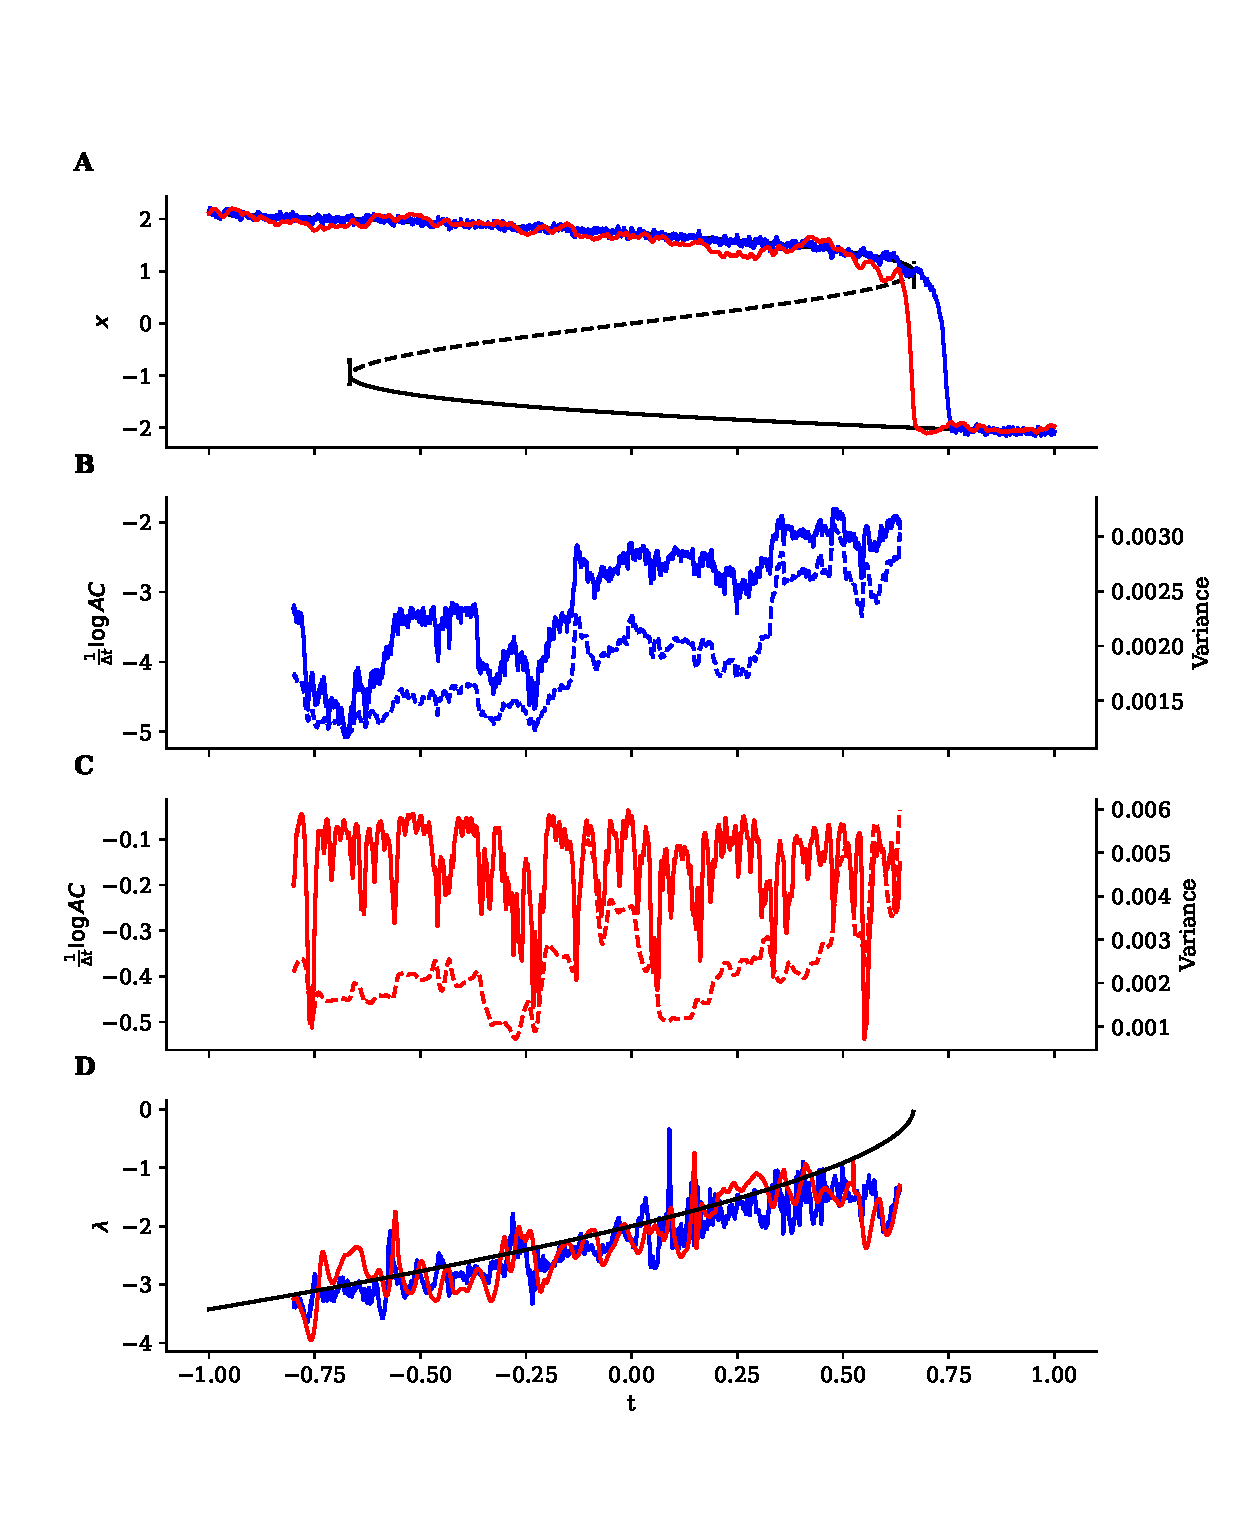
\includegraphics[scale=0.7,keepaspectratio]{figure1.eps}
\caption{Panel A shows two time series of system (\ref{eq:dynamical_system})--(\ref{eq:discretized_white_or_red_noise}), with $\mu(t)=t$ passing through a saddle node bifurcation at time $t=2/3$. 
  In the case of the blue curve the system
  is subject to white noise forcing ($r=0$), the red curve is subject to 
  red noise forcing ($r=0.99$). Panels B and C show the
  classic EWS for the case of white and
  red noise, calculated after a
  quadratic detrend in a window of width $0.2$ (in normalised time units or 500 data points).
  The AC is plotted with a solid curve and
  the variance with a 
  dashed curve.
  The white noise case shows clear EWS, 
  but the red noise case gives no indication of the approaching tipping point. Panel D shows $\lambda$ calculated from ROSA, after a
  qaudratic detrend in windows of length $0.2$, in the
  white (blue curve) and red (red curve) noise case. The solid black 
  line is the true value of $\lambda$. In both instances there
  is a clear Early Warning Signal.}
\label{fig:failure_of_ews}
\end{figure}

In this section, we demonstrate how conventional EWS may fail in the presence of autocorrelated  noise. Due to the fact that near a
saddle node bifurcation all dynamical systems with such a
bifurcation behave similarly\cite{guckenheimer2013}, we ought to
investigate the simplest bistable system exhibiting a saddle node
bifurcation. Hence, we examine the system 
\begin{equation}
    \label{eq:dynamical_system}
    \epsilon\dv{x}{t} =  x - \frac{1}{3}x^3 - \mu(t) + \eta(t),
\end{equation}
where we $\epsilon$ defines the timescale of the system, $\mu$ is a control parameter and $\eta$ provides the noise. We note that there is a saddle node bifurcation
when $\mu = 2/3$, corresponding to a tipping point where
$x$ transitions from a positive to a negative state. To ensure
$x$ remains in approximate equilibrium, we set $\epsilon$ to be small,
we take $\epsilon = 0.01$ throughout.


We define $\eta$ by the following Ornstein-Uhlenbeck 
process\cite{Uhlenbeck1930}:
\begin{equation}
\label{eq:white_red_forcing}
    \dv{\eta}{t} = \frac{r-1}{\delta t}\eta + \sqrt{\frac{1-r^2}{\delta t}} \xi
\end{equation}
where $\xi$ is the derivative of a standard Weiner process. 
This choice is more transparent when looked at in discrete form, with timestep 
$\delta t$:
\begin{equation}
    \label{eq:discretized_white_or_red_noise}
    \eta_{t+1} = r\eta_t + \sqrt{1-r^2} \epsilon_t
\end{equation}
with $\epsilon_t \sim \mathcal{N}(0,1)$. When $r = 0$, this is 
the conventional white noise assumed in most EWS
studies. However, as $r$ approaches unity the process becomes
more and more autocorrelated.

After discretizing with time step $\delta t = 0.0004$,
these equations are solved numerically using the 
Euler-Maruyama method\cite{Jacobs2010}.


\subsection{False Negatives}
As a system approaches a tipping point, the conventional
EWS suggest that the system should become more
autocorrelated. However, if the system is subjected to autocorrelated noise,
then this can act to mask the changes in the AC of the system so that such
changes are no longer detectable. Furthermore, decreasing variability in
the forcing can decrease the system variance even if the system is 
approaching a tipping point. This again acts to mask the approaching tipping point, which clearly poses problems for conventional
EWS as these would present a `false negative'.

To illustrate this, we set $\mu(t) = t$, so that system (\ref{eq:dynamical_system}) has
a tipping point at $t=2/3$ and calculate the conventional Early 
Warning Signals after detrending with a second order polynomial, plotted in Figure \ref{fig:failure_of_ews}.
Panel A of Figure \ref{fig:failure_of_ews} shows two time series of the 
state variable of (\ref{eq:dynamical_system}) approaching a tipping point.
The series are similar, except that one of them (blue) is subject to white noise ($r = 0$), 
while the other (red) curve is driven by red noise ($r = 0.99$). To
ensure the tipping occurs at a similar time in both
cases, we reduce the magnitude of the red noise by half.
Despite the qualitative similarity of the time series,
the classical EWS plotted in Panels B and C, are very different. To assist with comparisons to the method of this paper, we
plot $\frac{1}{\delta t}\log AC$ instead of the AC directly. However, this
transformation will have no effect on any trends.

The variance and AC show a clear rise in
the white noise case, giving a clear Early Warning Signal. 
Whereas, for the red noise case there is no trend in the AC. The 
variance shows both increases and decreases. A positive trend occurs near
the tipping point however this would give, if any, very little warning. Supplementary figure
S3 repeats this test for 1000 different noise realisations, showing the
challenge of getting EWS when the noise is very 
autocorrelated.
%It is difficult to see any trend in the red noise case; to the extent a trend exists it is negative. There is an increase in variance before the 
%tipping, but in contrast to the white noise case this only
%occurs just before the tipping.


\subsection{False Positives}
An additional problem with assuming the system is subject to stationary white noise is that it also implies that the
variability and AC of the forcing is constant over time. 
However in the case of 
climate change, it is likely that the variability of the forcing,
such as temperature, will change\cite{Huntingford2013}. 
Increasing the variability, such as in \cite{Boers2021a}, of the forcing will increase the variance of the system even
if the system is not approaching a tipping point. This is an example of a false
alarm (i.e.\ a false positive). 

\begin{figure}
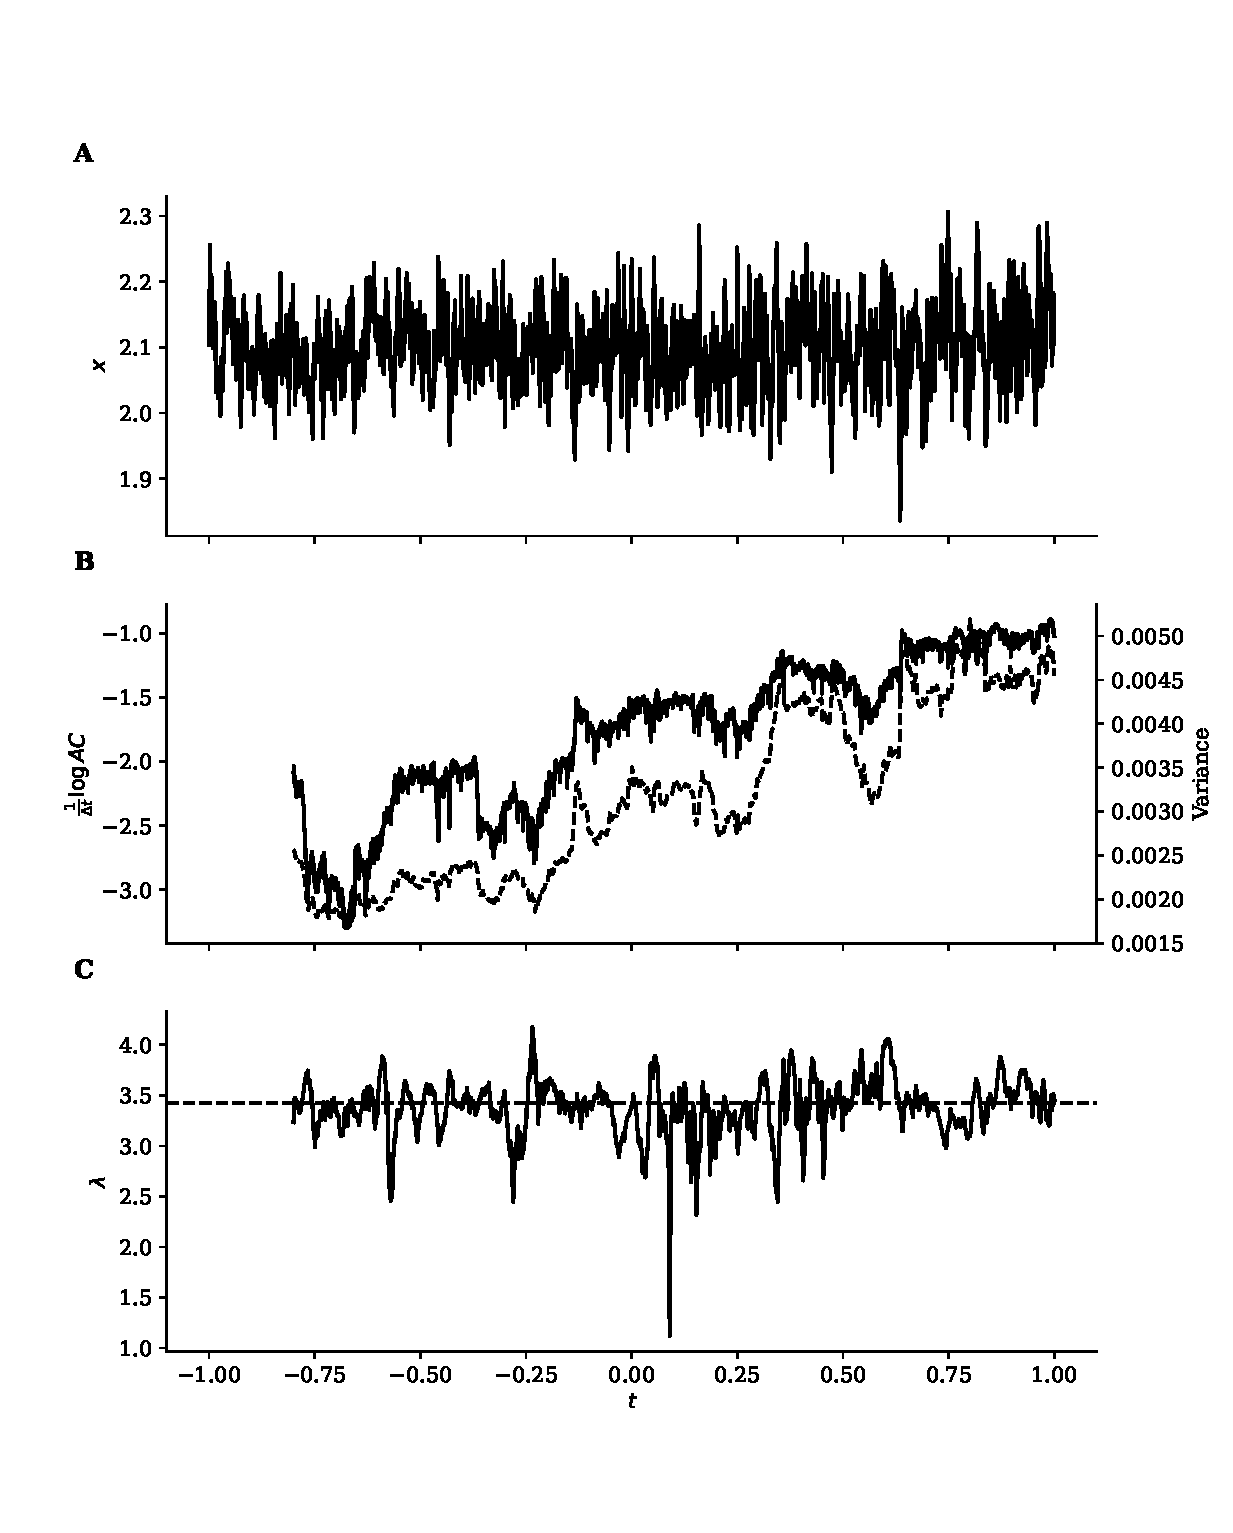
\includegraphics[width=\textwidth,keepaspectratio]{figure2.eps}
\caption{Panel A shows a time series obtained by integrating Equation (\ref{eq:dynamical_system}) with $\mu = -1$ when subject to
  noise described by (\ref{eq:white_red_forcing}) where the
  value of $r$ linearly increases from $r=0.2$ to $r=0.7$. Panel B 
  shows the classic Early Warning indicators: AC in the solid
  line and variance in the dashed line. They falsely indicate a
  tipping point is approaching. In panel C we plot $\lambda$ obtained
  from ROSA, with the true value plotted in the dashed line. It shows
  no overall trend hence correctly avoiding the false positive.}
\label{fig:changing_forcing}
\end{figure}


An example of this phenomenon is plotted in Figure
\ref{fig:changing_forcing}. We have integrated 
(\ref{eq:dynamical_system}) with $\mu = -1$, hence there is no 
tipping point. The stochastic forcing $\eta$, described by (\ref{eq:white_red_forcing}), has its $r$ value
linearly increasing
from $r=0.2$ at $t=-1$ to $r=0.7$ at $t=1$. The state
variable is plotted in Panel A. Although there is no
tipping point crossed, because the forcing is becoming 
increasingly autocorrelated, the classical early warning indicators 
(Panel B) falsely suggest a tipping point is approaching.

\section{Theory}
\label{sec:theory}
These issues motivate creating a generic early warning signal, 
for B-tipping, that is 
independent of the form of external forcing. Conceptually,
the method is to `divide out the' the noise process.
While it is not clear
how to do this directly from the time series, we show that this can be achieved if we move
to the frequency domain, where it is has been shown to be possible
to extract estimates of distances to bifurcation 
points\cite{Kleinen2003}, by taking a Fourier Transform of the data. 
Under white noise forcing, it is found that the spectrum reddens\cite{Kefi2014,Dakos2012c}, we look at the case where the forcing 
can mask this reddening.

We begin by modelling a tipping element with a state variable $y$ that evolves in time $t$, and depends on a slowly evolving parameter $\mu$.  The tipping point occurs when $\mu=\mu_c$.
We can  write this generically as:
\begin{eqnarray}
\label{eq:full_syste}
    \dv{y}{t} &= f(y,\mu),\\
    \dv{\mu}{t} &= \epsilon g(y,\mu).
\end{eqnarray}
for some functions $f$ and $g$, and $\epsilon \ll 1$.
As $\epsilon g(y,\mu)$ is small, we can use the theory of fast-slow systems\cite{Kuehn2011} to reduce to a one
dimensional dynamical system depending only on the parameter $\mu$:
\begin{equation}
  \label{eq:1d_dynamical_sys}
  \dv{y}{t} = f(y,\mu).
\end{equation}
At this point, we apply an additional time-dependent perturbation $\xi(t)$, which can have a stochastic component. We now have:
\begin{equation}
  \label{eq:1d_dyn_sys_forced}
  \dv{y}{t} = f(y,\mu) + \xi(t).
\end{equation}
The classical theory of EWS assumes $\xi$ is a white noise process, however we make no such restriction. It may have both
deterministic and stochastic components, we only require that its 
Fourier Transform exists.

Linearising about a quasiequilibrium, $x^*$, (i.e. that is evolving on the slower timescale), we write
$y(t) = x^* + x(t)$ to give:
\begin{equation}
  \label{eq:linearised}
  \dv{x}{t} \approx -\lambda x + \xi(t),
\end{equation}
where $\lambda = -f'(x^*,\mu)$ and the prime denotes a derivative with respect to $x$. 
Physically, $\lambda$ represents the rate at which the system returns to equilibrium after
a disturbance, and thus characterises the resilience of a system. Held and Kleinen\cite{Held2004} developed a technique to estimate $\lambda$
under the assumption that $\xi$ is Gaussian white noise. Here, we will
relax that assumption.
When $\mu \rightarrow \mu_c$, which is to say that the system approaches
the tipping point, then it turns out that $\lambda \rightarrow 0$\cite{guckenheimer2013}. This is the phenomenon of critical slowing down. Our aim is to therefore
identify changes in $\lambda$, and in particular discover any evidence of a decrease which would suggest an approaching tipping point, and
to do this in a way that is not dependent on $\xi$ being white noise. To achieve this, we move to the frequency domain.

We denote the Fourier transform of a function with a tilde, so that when taking the Fourier transform of (\ref{eq:linearised}) we have
\begin{equation}
  \label{eq:fourier_transformed}
  i\omega \tilde{x}(\omega) = -\lambda \tilde{x}(\omega) + \tilde{\xi}(\omega).
\end{equation}
We can rearrange Equation~(\ref{eq:fourier_transformed}), and then take the squared modulus to get:
\begin{equation}
  \label{eq:power_spectra}
  |\tilde{x}(\omega)|^2 = \frac{|\tilde{\xi}(\omega)|^2}{\omega^2 + \lambda^2}.
\end{equation}
We now define the ratio of spectra (ROSA)
$R(\omega) = |\tilde{x}/\tilde{\xi}|^2$ so that
\begin{equation}
    \label{eq:power_spectrum_indep}
    R(\omega) = \frac{1}{\omega^2 + \lambda^2}.
\end{equation}
We note that by construction $R$ takes on a universal form for any 
forcing process,
hence estimates of $\lambda$, and thus of the 
distance to the tipping point, can be made from $R$ regardless 
of whether the noise is time correlated or not. It also suggests an
Early Warning Signal method.

The method is as follows.
We now take a moving window of length $\tau_w$, smaller than the slow timescale $1/\epsilon$, but of sufficient
length that we can calculate the power spectrum of $x$, i.e. $|\tilde{x}(\omega)|^2$, and also of
$\xi$, i.e. $|\tilde{\xi}(\omega)|^2$. With the knowledge of these power spectra, we perform a least-squares fit of equation~(\ref{eq:power_spectrum_indep}) to obtain an estimate for $|\lambda|$.  We then consider how $|\lambda|$ varies over longer timescales, i.e. of
size $1/\epsilon$, to see if its value changes. 
If our estimate for $|\lambda|$ is decreasing towards zero in time this implies that a tipping point is approaching. 

\subsection{Choosing $\xi$}
Unlike most EWS, our ROSA method requires knowledge of
the driving process that controls the variability of the system.
Therefore, using this method requires an understanding
of the system. Furthermore the system must be of sufficient temporal resolution such that 
both $x$ and $\xi$ can be measured. If $\xi$ is not chosen
correctly then changes to the calculated $\lambda$ could be driven
by changes to the incorrectly chosen $\xi$, rather than a 
tipping point. 

We argue that these requirements are not too restrictive, at least in the 
case of EWS for transitions caused by contemporary
climate change. Many different Earth System quantities are regularly 
measured and many processes are understood. Furthermore to help 
guard against choosing the wrong $\xi$ it could first be tested in an Earth System Model (ESM). Note however that ESMs represent tipping elements 
poorly, with little agreement between models\cite{Drijfhout2015}.


\section{Test in Simple Models}
We examine this ROSA method using the two test cases considered earlier in 
section \ref{sec:failure}; namely its ability to avoid 
false positives and false negatives.
We calculate the power spectra of $x$ and $\eta$
using Welch's method\cite{Welch1967} after a quadratic 
detrend in moving windows of length $0.2$. We perform a least
squares fit to
(\ref{eq:power_spectrum_indep}) and extract $\lambda$. We plot
the results in panels D and C of Figures 
\ref{fig:failure_of_ews} and \ref{fig:changing_forcing} respectively.

\subsection{Avoiding False Negatives}
In Figure \ref{fig:failure_of_ews} we plot the case
where the system is approaching a tipping point
subject to white or red noise. Panel D provides
the value of $\lambda$ estimated from ROSA and shows a clear
rise towards zero in both the white and red noise case indicating
a successful warning, in contrast to the classical indicators. Furthermore, both the
white and red noise estimates lie close to the true value of 
$\lambda$, plotted in the black curve.

\subsection{Avoiding False Positives}
In Figure \ref{fig:changing_forcing} we look at the case where the 
system is not approaching a tipping point, but due to a reddening of 
the noise process the classic Early Warning Indicators give a 
false positive. In Panel C we plot $\lambda$ obtained from ROSA, which stays constant and close to the true value (plotted in the dashed line). ROSA therefore avoids a false positive in this case.




\section{Comparison to alternative methods}
Recently, Boers\cite{Boers2021a} introduced a new technique,
to avoid the problems introduced by noise that isn't white.This was
more rigorously analysed by Boettner and Boers\cite{Boettner2022}. The
technique, which we refer to as the BB method, is essentially a way of
regressing $\dot{x}$ against $x$, to give an estimate for $\lambda$. 
This requires a model for the noise, for example that it is
generated by an Ornstein-Uhlenbeck process. Significantly, the BB method makes a quasi-static assumption, such that the parameters of the noise
model are assumed to be fixed in each window (although can change between windows). On the other hand,
ROSA does not have such a restriction because the noise is analysed directly.

We compare the BB method with ROSA for a system defined by
(\ref{eq:dynamical_system}). We set $\mu  = t$ so that the system
reaches a tipping point at $t=2/3$. Furthermore we linearly decrease
$r$ from $r=0.99$ to $r=0.0$ between $t=-1$ and $t=1$.
This decreasing AC of the
noise can feed through into the system's AC, thus masking
the conventional EWS. This test therefore
combines the challenges of predicting a tipping point with dealing
with non-stationary noise.

Both methods give estimates for $-\lambda$, which should rise
to zero as the tipping point is approached. To compare the 
rise we compute a running Kendall $\tau$\cite{Wilks2019} for all data points up to
that time. This quantity, bounded 
between $-1$ and $1$ gives a measure of whether a sequence is 
increasing or decreasing. A strongly positive $\tau$ suggests a tipping point is approaching, and a strongly negative $\tau$ suggests one is not. To give the best Early Warning $\tau$ should become
large as long before the tipping point as possible.


We compute this for $10$ noise realisations and plot the output 
in Figure \ref{fig:boers_method}. Both indicators show a positive 
$\tau$ near the tipping point. However, ROSA becomes positive substantially earlier than the BB method and there is less variance in the $\tau$ values for the ROSA method, as required for a more reliable early warning indicator. This is indicative of an earlier and stronger warning than the BB method. 

Nevertheless, the BB method has its advantages.
It is flexible and straightforward to modify to different noise
models and in many cases gives a good Early Warning Signal 
ahead of the tipping point. Its principle advantage
over ROSA is that an explicit time series of the forcing is not required to use it. As a result, ROSA and BB should be seen as complementary methods: 
where data is scarce such as in paleoclimate studies, BB is more suitable but 
for contemporary climate change where the earliness of the warning is 
important ROSA is more suited.

\begin{figure}
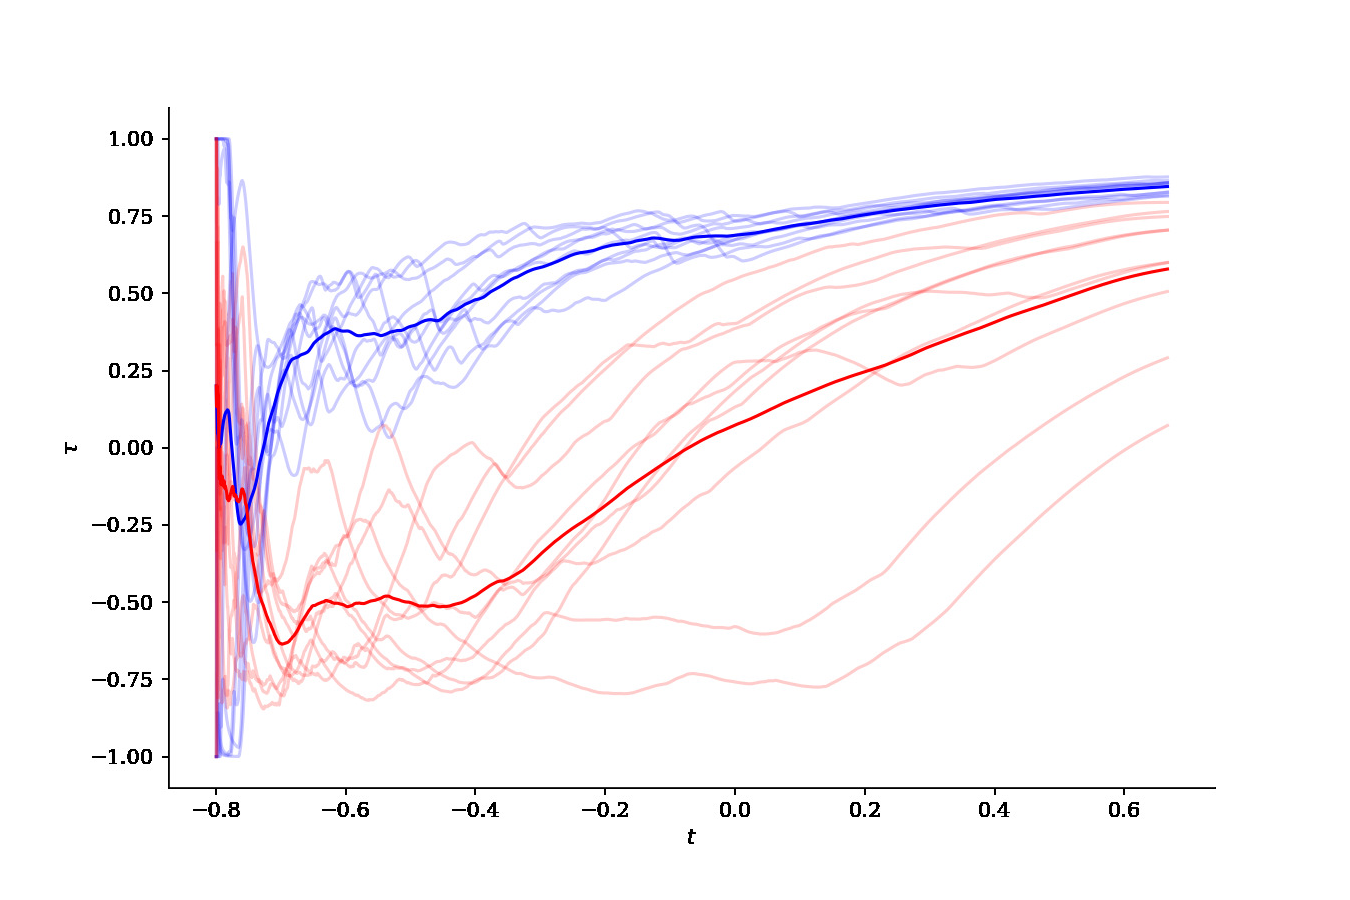
\includegraphics[width=\textwidth,keepaspectratio]{figure3.eps}
\caption{A plot of running Kendall $\tau$ values as a function of time for the ROSA (blue) and BB (red) methods. Individual realisations are plotted in faint lines and the mean value is plotted in the stronger colour. ROSA gives an earlier and more reliable warning than the BB 
method.}
\label{fig:boers_method}
\end{figure}

\section{Complex Models}
The verification of our proposed early warning system with relatively simple conceptual models is important.
However, the majority of components of the Earth System are complex, requiring highly detailed numerical models to emulate them. Hence, it is 
desirable to see if the technique is still successful in the case of
a more complex model. The dimensionality of such models can be very high, due to their spatial extent and related heterogeneity, and 
because the forcing $\xi$ is uncertain and may not be a single dominant forcing,  but instead a combination of external fluctuating drivers. These individual components, when combined, make-up `full-form' Earth System Models (ESMs).

%Fortunately, there are many such complex models to choose from.
There are a very large number of ESMs available, and additionally a substantial number of attributes of the Earth system amenable to investigation. Here we 
examine Amazon forest dieback in state-of-the-art ESMs from the Coupled Model Intercomparison  Project - Phase 6 (CMIP6)\cite{Eyring2016} database. Recently,
five (EC-Earth3-Veg, GFDL-ESM4, NorCPM1, SAM0-UNICON and TaiESM1) of seven models, which possess a Dynamic Global Vegetation Model
(DGVM), have been shown to feature abrupt local Amazon dieback shifts (in the IPCC defined North South American region) in an idealised run of increasing CO$_2$ by 1\% per year\cite{Parry2022}.
%(Is this correct???).The model UKESM1-0-LL also has a DGVM but does not show Amazon dieback.
The algorithm used in the study (and here) detects an abrupt shift if the following three criteria are satisfied: 1) the abrupt change is fast such that vegetation carbon drops by at least 2 \si{\kilogram\carbon\per\meter\squared} in a 15-year period, 2) the abrupt shift contributes to at least a quarter of the total change in the run, and 3) the mean annual rate of change is more than three times the variability of the rate of changes observed in the unforced control run. 
%(is there a citation for it? tipping point = abrupt shift - 5 years) 

In every grid point identified as containing an abrupt shift, the time series of monthly vegetation carbon had its nonlinear trend and seasonal cycle removed
%This data was then deseasonalised and detrended 
using the seasonal and trend decomposition using
Loess (STL) method\cite{Cleaveland1990}. In 
windows of length 50 years the conventional EWS and ROSA were calculated.
We choose the \si{2\meter} air temperature as our forcing variable, which
was detrended similarly to the vegetation carbon. 

Although this choice of forcing variable is unlikely to capture all aspects
of the forcing, there is a known connection between temperature and Amazon 
dieback. For example, increases in the temperature seasonal cycle amplitude reveal declines in the evaporative fraction and hence a drying over the Amazon basin\cite{Ritchie2022}. Moreover, high sensitivities of the temperature seasonal cycle to global warming are more likely to incur abrupt forest dieback events\cite{Parry2022} in CMIP6. Furthermore there is a link between temperature anomalies and Amazon productivity\cite{Boulton2013}. Therefore, the air temperature plays an important role in controlling the resilience of the forest.

For each of these indicators, we calculate the Kendall $\tau$ statistic for the
20 year period prior to the abrupt shift. If that $\tau$ is above some threshold, we 
count that as a detection. As we expect the variance in vegetation carbon to be higher 
in a high CO$_2$ world, we only take increases in variance as a detection if
the AC is not decreasing. The results, as a function of threshold value
is plotted in figure \ref{fig:complex_test}.

We note that the algorithm will, in addition to examples of B-tipping, detect examples
of N-tipping and rapid change which is not a true tipping point. As a result, no 
EWS will successfully detect all abrupt shifts. This also means that some
of the warning signals will be false positives. However this possibility
affects all the EWS so the comparison remains fair. All three EWS are capable
of detecting substantial proportions of the identified abrupt shifts. Overall, we see that ROSA outperforms the traditional EWS. For individual models,
ROSA detects more abrupt shifts than the AC alone and is often better than the 
variance. Hence, for most of the CMIP6 models considered, ROSA is able to give a more robust
early warning for abrupt shifts.

\begin{figure}
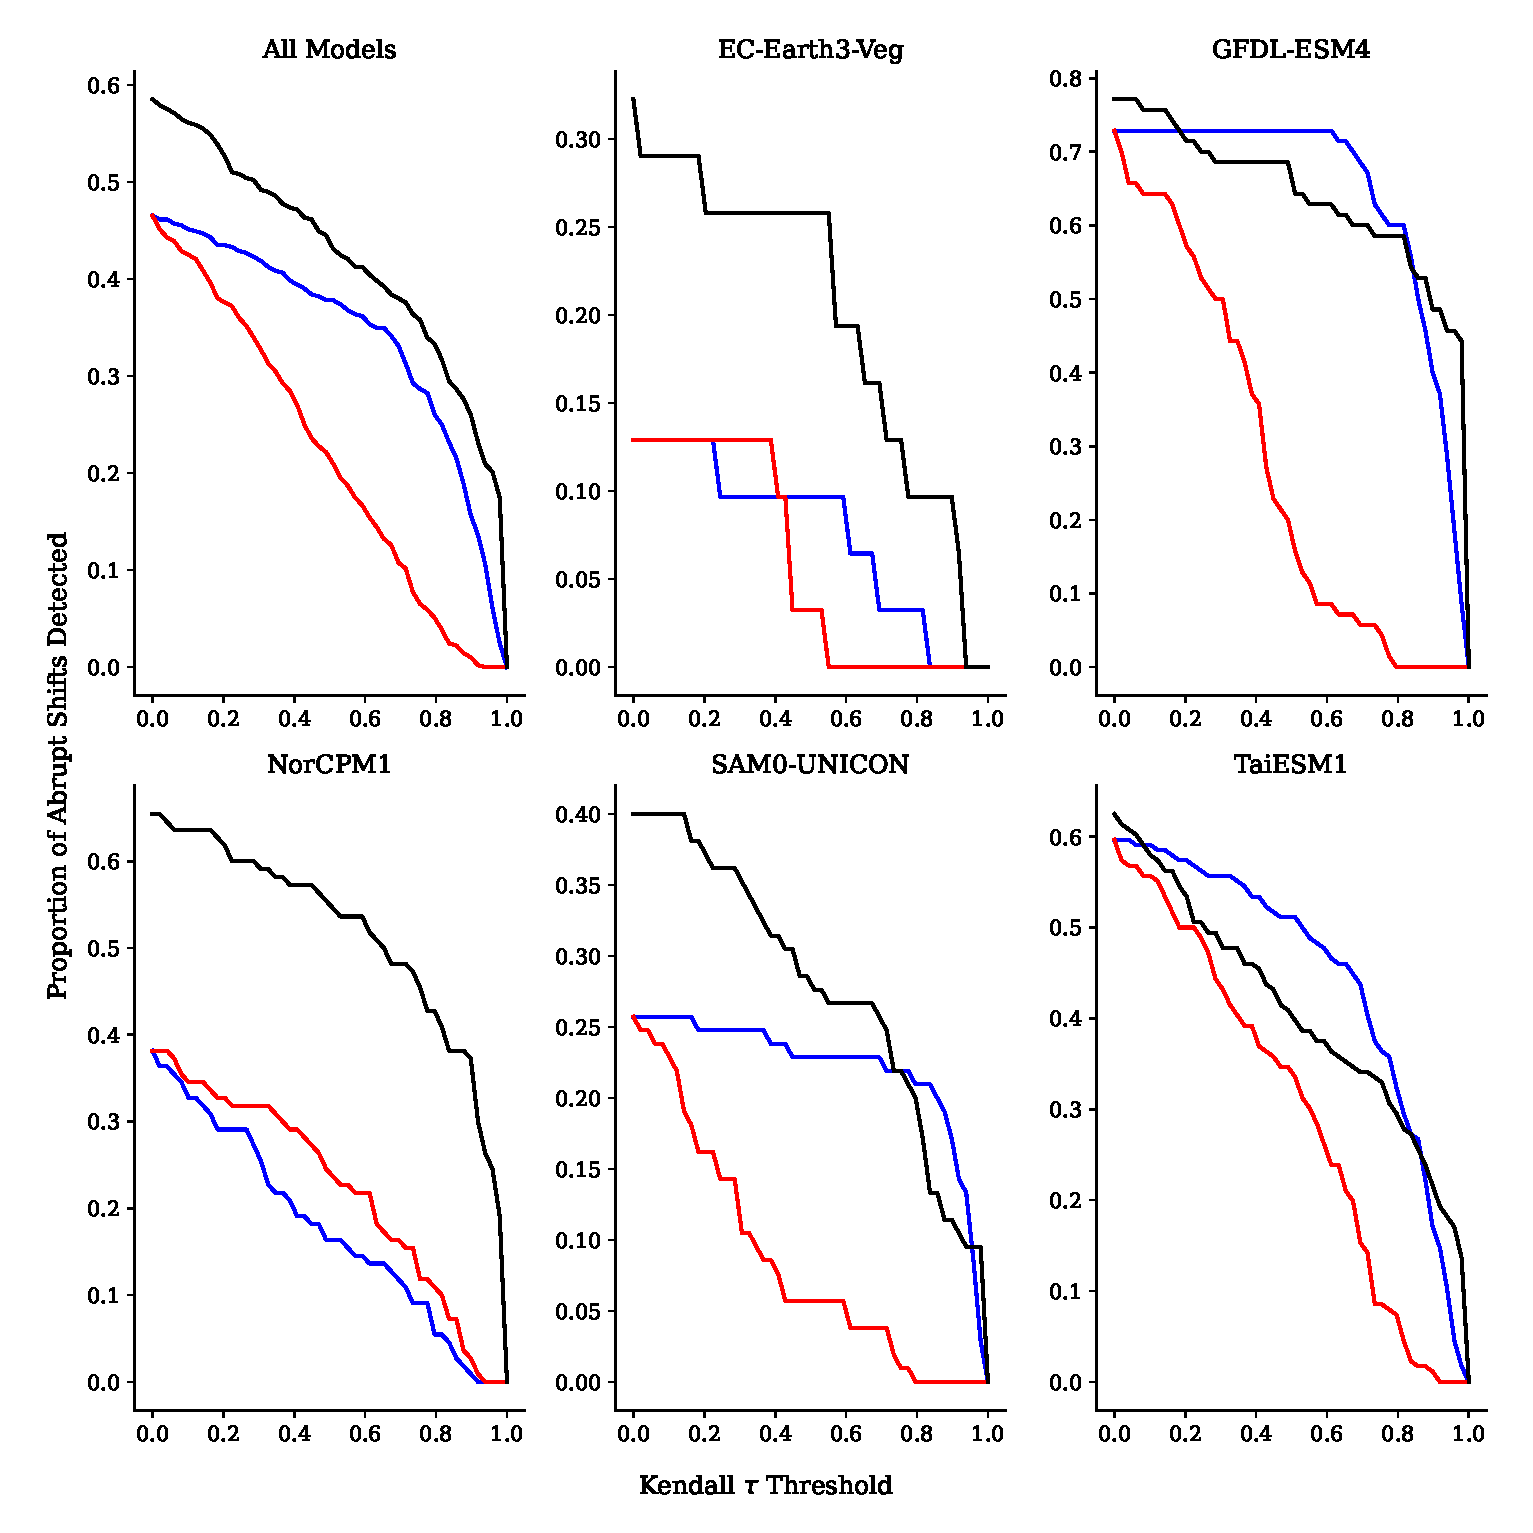
\includegraphics[scale=0.6,keepaspectratio]{figure4.eps}
\caption{The proportion of abrupt shifts in Amazon vegetation carbon
detected, as a function of threshold Kendall $\tau$ for three EWS across 5 ESMs. The blue line is the variance,
the red is the AC and the black is ROSA.}
\label{fig:complex_test}
\end{figure}



\section{Discussion and Conclusions}
The potential presence of tipping points in the climate system remains of particular concern. 
Tipping points imply that relatively small changes in forcing could trigger
disproportionately large (and possibly irreversible) changes.
For these reasons, it is essential to develop
statistics that can identify approaching tipping points.

Although there has been much work on EWS for Tipping Points,
this has tended to focus on the simple case that the system is subject to additive white noise. 
In this paper we have shown how EWS can be generalised to deal with more general noise characteristics. By normalising the power spectrum of the forcing, we are able to extract a 
time-evolving parameter $\lambda$, which robustly approaches zero as a tipping point is approached.  

Approximating the driving noise as white is reasonable when $r$ is 
small or when the window length can be chosen to be long relative to the 
noise's decorrelation time. In these instances, conventional EWS will be useful. ROSA is most applicable to the cases where this choice is not
possible. This is relevant to anthropogenic climate change given that the changes are fast.

Our work relies on a couple of  key assumptions: (a) that there is a separation of timescales; and (b) that the power spectrum of the forcing and the system is known. Assumption (b)
requires having data for a sufficiently long period of time, which may 
prove challenging in practise. Assumption (b) is notable as other EWS, like the BB technique, do not require the forcing to be known.
Although assumption (a) is typically
assumed when dealing with EWS, its applicability
to the rapidly changing modern climate is still an open 
question.
As a result, future work should investigate EWS for systems without this timescale separation. Nevertheless, we believe our approach represents an increase in the flexibility and generality of EWS for tipping points in a changing climate. 

\section*{Data Avaliablity}
The code used to produce the figures in this paper can be found at \texttt{https://github.com/josephjclarke/BeyondWhiteNoiseEWS}.



